\capitulo{5}{Aspectos relevantes del desarrollo del proyecto}
En este apartado, se detallan los aspectos más relevantes que han ocurrido durante el desarrollo del proyecto, así como la manera en la que el proyecto ha sido realizado para cumplir los objetivos propuestos.

\section{Limpieza de datos}
Como ya se ha explicado en el punto \ref{limpieza}, los datos obtenidos pueden contener ruido que perjudique la tarea que se quiere realizar, en este caso, la clasificación. Por esta razón, es necesario corregirlos de alguna manera.

\subsection{Filtro de Savitzky-Golay}
En el apartado de conceptos teóricos \ref{savgol}, ya se mencionó el filtro de Savitzky-Golay, con el que se podían mejorar las gráficas representando los resultados obtenidos.

Estos resultados contienen ruido tanto por el propio pulso de la mano como por la biblioteca que detecta la mano, por lo que su representación en ocasiones muestra demasiados máximos o mínimos parecidos, confundiendo los valores reales.

\subsection{Distancias} 
Las distancias ya obtenidas no muestran la distancia  real, por lo que es necesario realizar un paso previo antes de calcular el resto de características que dependen de la distancia. 

Dado que la pinza cerrada es el momento en el que menos distancia hay, lo lógico sería pensar que esta distancia es 0, sin embargo, esto no ocurre debido a la localización de los puntos de los dedos. Estos puntos no están justo en la yema de los dedos, donde la pinza se cierra, sino que están en el centro del dedo, por lo que la distancia entre esos puntos nunca será 0, aunque sí muy próxima, es decir, las distancias mínimas nunca serán 0. Al igual que sucede con las distancias mínimas, también las distancias máximas se ven afectadas, y en general, todas las distancias. Por esta razón, se realizan nuevamente las restas de los máximos y mínimos de las distancias anteriormente calculadas para que los nuevos mínimos alcancen valores mucho más cercanos al 0. 

Para comprender esto mejor, se va a suponer que una distancia mínima entre los dos dedos es de 0,051 y una distancia máxima es de 0,376. Al igual que el 0,051 no es el mínimo real, pues lo lógico sería que fuese 0, la verdadera amplitud máxima tampoco sería real, pues debería contar desde el 0. Para obtener la distancia real habría que obtener la diferencia entre el máximo y el mínimo, para conocer la distancia que les separa, es decir, la amplitud de la pinza, que sería 0,325. 

Realmente, todos los puntos no están recogiendo valores reales, sin embargo, dado que sólo interesa recoger la distancia máxima, únicamente se realiza la diferencia entre máximos y mínimos.

\section{Obtención de características}
En este punto se trata de buscar otros datos que caractericen a los vídeos con el fin de poder realizar una clasificación. Habrá datos calculados y datos que ya vienen dados porque no se pueden calcular, como la mano, la edad o el sexo.

\subsection{Amplitud}
Esta característica es la más evidente ya que, generalmente, los pacientes con Parkinson ven dificultad a la hora de abrir y cerrar la mano hasta su punto máximo.

Para su extracción, en primer lugar, se han recogido los máximos y mínimos de la gráfica de los 5 primeros movimientos y de los 5 últimos. Después, estos datos se normalizan para que no afecte la distancia de la mano a la cámara. Esta normalización se obtiene de la siguiente fórmula:

\begin{equation}
	X_{normalizada} = \frac{X_{actual} - X_{mínima}}{X_{máxima}-X_{mínima}}
\end{equation}

Para la extracción de las distancias, tanto la original como la normalizada, tan solo hay que restar el mínimo con el máximo correspondiente. 

\subsection{Tiempo}
Otra de las características que podrían afectar a una persona que tiene Parkinson es cuánto tardaría en realizar el movimiento de pinza, ya que, en un principio, aquellos que padezcan la enfermedad tardarán más.

Para ello, se ha realizado la diferencia entre un máximo y el mínimo correspondiente. En este caso se ha utilizado como unidad temporal el número de fotogramas entre ambos puntos, ya que, a más lentitud, más fotogramas habrá de diferencia y viceversa.

Sin embargo, esta medida resulta no ser suficiente porque no se tiene en cuenta cuánto se ha abierto la pinza, es decir, alguien que abra la pinza lentamente y hasta la mitad tardará el mismo tiempo que alguien que la abra más rápido y hasta el máximo.

\subsection{Velocidad}
Para solucionar el problema anterior, se puede utilizar la velocidad. Esto es, calcular la distancia recorrida por unidad de tiempo, por lo que dependiendo de cuánto se recorra y en cuánto tiempo, una persona tendrá más velocidad o no.

En una primera instancia, una persona que padece Parkinson, dada su reducida movilidad, pese a abrir la pinza hasta su punto máximo, lo más seguro es que lo hiciera de forma más lenta que otra persona sin Parkinson.

Esta velocidad se calcula realizando la división de la diferencia normalizada entre un máximo y un mínimo (\textit{i. e.} la amplitud ya calculada), entre el tiempo que les separa a ambos puntos (\textit{i. e.} el tiempo ya calculado).

Para este trabajo, se ha calculado la velocidad media de cada vídeo.

\subsection{Mano derecha o izquierda}
Como añadido, también se ha tenido en cuenta si la mano es derecha o izquierda. En un principio, podría resultar interesante conocer cuál es la mano que más dificultades tiene a la hora de realizar el movimiento, aunque tampoco resulta fundamental para clasificar. Esta característica no es calculada, sino que viene dada con el vídeo.

\subsection{Sexo}
El sexo de la persona podría servir para clasificar las personas con y sin Parkinson. Como se ha mencionado en la introducción de este documento, el Parkinson es más propenso a aparecer en hombres, por lo que, en primera instancia, podría haber más hombres con Parkinson que mujeres, o lo que es lo mismo, más mujeres sin Parkinson que hombres, lo cual podría ayudar a la hora de clasificar. Al igual que con la mano, esta característica no es calculada, sino que viene dada con el vídeo.

\subsection{Edad}
De forma similar a lo que ocurre con el sexo, el Parkinson es más propenso en personas mayores, de 60 años, por lo que la edad también podría resultar interesante a la hora de clasificar.

Sin embargo, hay que tener cuidado con los ejemplos a la hora de entrenar modelos, ya que el sistema podría aprender que todos los menores de, por ejemplo, 30 años nunca tendrán Parkinson, cuando esto no es cierto. Esto dependerá de la muestra de entrenamiento, ya que si hay pacientes de diversas edades con Parkinson, el modelo realizará la predicción teniendo en cuenta también esos casos. 

Pese a poder ser interesante, esta característica con los datos utilizados no mejora los resultados, por lo que finalmente no será utilizada. Esta característica tampoco es calculada, también viene dada con el vídeo.

\section{Resultados} \label{resultados}
Para obtener mejores resultados es importante que el conjunto de datos utilizado para entrenar el modelo esté equilibrado. Sin embargo, estos resultados no son tan buenos como se podría esperar, aunque sí se obtiene una diferencia entre aquellos con y sin Parkinson. Este conjunto de datos debería contar con más ejemplos para que el clasificador fuese capaz de distinguir diferentes niveles de Parkinson entre dos pacientes.

Para conocer cuál es el clasificador que mejor predice, se ha realizado un estudio de los resultados, utilizando las métricas ya explicadas en el apartado \ref{medidas}. Además, también se ha realizado un estudio de tiempos, para conocer cuál es el clasificador más rápido.

\subsection{Predicción}
Para realizar la predicción, se han utilizado los clasificadores ya explicados en el apartado \ref{clasificadores}, donde cada columna se corresponde a las siglas de cada clasificador. Se han descartado algunas de las características obtenidas como las amplitudes sin normalizar, la edad o el tiempo ya que empeoraban la clasificación. Además, se ha utilizado una validación cruzada de 2 divisiones y 5 repeticiones, obteniéndose los siguientes resultados:

\begin{table}[h]
	\begin{center}
		\begin{tabular}{ l l l l l l l l }
			\toprule
			\textbf{Medidas} & \textbf{RF} & \textbf{k-NN} & \textbf{AD} & \textbf{NBG} & \textbf{SVM} & \textbf{NB} & \textbf{Dummy} \\ \midrule
			accuracy & 0,719 & 0,544 & 0,669& 0,4888 & 0,562 & 0,575 & 0,562 \\
			Matt. corr. coeff. & 0,435 & 0,084 & 0,315 & -0,015 & 0,013 & 0,075 & 0 \\ 
			f1 & 0,75 & 0,577 & 0,71 & 0,482 & 0,707 & 0,708 & 0,72 \\
			ROC AUC & 0,776 & 0,547 & 0,663& 0,467 & 0,57 & 0,521 & 0,5 \\
			g mean & 0,706 & 0,522 & 0,609 & 0,468 & 0,056 & 0,252 & 0 \\ \bottomrule
		\end{tabular}
		\caption{Tabla con las medidas y clasificadores utilizados.}
		\label{tab:medidas}
	\end{center}
\end{table}

Lo más destacable de estos resultados es el área bajo la curva ROC (\textit{ROC AUC}) y la precisión (\textit{accuracy}), siendo el clasificador Random Forest el mejor en ambos.

El área bajo la curva ROC del clasificador es 0,776, y significa que gran parte de los ejemplos los diferencia correctamente, sin confundir una clase con la otra. En general todos los clasificadores realizan una clasificación bastante decente, ya que diferencian más o menos bien los ejemplos de una clase de los de la otra, a excepción del clasificador Naive Bayes Gaussiano. Si este clasificador se utilizara a la inversa, esto es, cuando prediga sí decir no y viceversa, tendría un valor de 0,533 ($1 - 0,467$), que aunque no sea demasiado optimista, sería mejor que utilizarlo tal y como está.

Por otro lado, la precisión indica que hay un 71,9 \% de ejemplos bien clasificados, teniendo en cuenta que además los está identificando bien. 

\subsection{Tiempos de entrenamiento}
Se ha realizado un estudio de los tiempos que tardan en entrenar los modelos. Para ello, se han realizado 10 ejecuciones con cada modelo para conocer una aproximación del tiempo que tardan en entrenar, donde se han obtenido los siguientes resultados en segundos:

\begin{table}[h]
	\small
	\begin{center}
		\begin{tabular}{ l l l l l l l l }
			\toprule
			\textbf{Ejecuciones} & \textbf{RF} & \textbf{k-NN} & \textbf{AD} & \textbf{NBG} & \textbf{SVM} & \textbf{NB} & \textbf{Dummy} \\ \midrule
			1 & 0,32934 & 0,00397 & 0,00347 & 0,00294 & 0,005 & 0,00505 & 0,00046 \\
			2 & 0,33381 & 0,00391 & 0,00297 & 0,00347 & 0,00561 & 0,00449 & 0 \\ 
			3 & 0,28417 & 0,00319 & 0,00198 & 0,00347 & 0,00546 & 0,00496 & 0,0006 \\
			4 & 0,32095 & 0,00362 & 0,00347 & 0,00347 & 0,00493 & 0,00534 & 0 \\
			5 & 0,26536 & 0,00248 & 0,00198 & 0,00542 & 0,00592 & 0,00496 & 0,0005 \\
			6 & 0,32885 & 0,00149 & 0,00294 & 0,00347 & 0,00545 & 0,00465 & 0 \\
			7 & 0,33331 & 0,00248 & 0,00397 & 0,00298 & 0,00552 & 0,00493 & 0,0005 \\
			8 & 0,32438 & 0,00248 & 0,00298 & 0,00397 & 0,00397 & 0,00496 & 0 \\
			9 & 0,245 & 0,00199 & 0,00252 & 0,00446 & 0,00455 & 0,00298 & 0,0005 \\
			10 & 0,28023 & 0,00244 & 0,00296 & 0,00447 & 0,00528 & 0,00308 & 0,0005 \\ \midrule
			Media & 0,30454 & 0,0028 & 0,00292 & 0,00381 & 0,00517 & 0,00454 & 0,00031 \\ \bottomrule
		\end{tabular}
		\caption{Tabla con los tiempos de entrenamiento de cada modelo con las 10 ejecuciones.}
		\label{tab:tiempos_entrenamiento}
	\end{center}
\end{table}

Además, se muestran estos datos en formato de gráfica en la figura \ref{fig:grafico_entrenamiento}.

\begin{figure}[ht]
	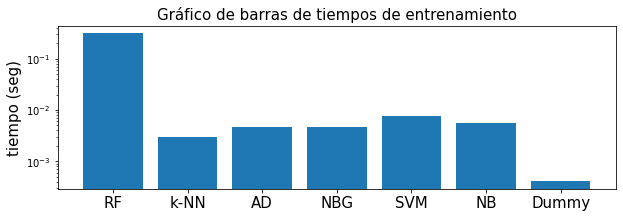
\includegraphics[width=1\textwidth]{grafico_entrenamiento}
	\caption{Gráfico de barras con los tiempos medios de entrenamiento de cada modelo.}
	\label{fig:grafico_entrenamiento}
\end{figure} 

Viendo los resultados, se puede observar que el clasificador que más destaca frente al resto es el Random Forest. Esto se debe a cómo se construye el clasificador. Dado que Random Forest es un \textit{ensemble}, es decir, que está formado por varios clasificadores, en este caso, árboles de decisión, tiene que realizar la construcción de cada árbol de decisión para construir el clasificador completo. 

En la otra parte está el clasificador Dummy. Como ya se ha comentado, este clasificador realiza una predicción de la clase mayoritaria, es decir, no necesita tomar decisiones internas sobre qué clase asignar a la instancia que se está clasificando, por lo que no requiere apenas tiempo para construir el clasificador.

\subsection{Tiempos de predicción}
También se ha realizado un estudio de los tiempos que tardan en predecir los modelos. Al igual que sucedía con el estudio anterior, se han realizado 10 ejecuciones con cada modelo para conocer una aproximación del tiempo que tardan en predecir, donde se han obtenido los siguientes resultados:

\begin{table}[h]
	\small 
	\begin{center}
		\begin{tabular}{ l l l l l l l l }
			\hline
			\textbf{Ejecuciones} & \textbf{RF} & \textbf{k-NN} & \textbf{AD} & \textbf{NBG} & \textbf{SVM} & \textbf{NB} & \textbf{Dummy} \\ \hline
			1 & 0,02381 & 0,00502 & 0,00149 & 0,00301 & 0,00397 & 0,00285 & 0,00053 \\
			2 & 0,03476 & 0,00524 & 0,00099 & 0,00244 & 0,00328 & 0,00347 & 0,00099 \\ 
			3 & 0,01885 & 0,00496 & 0,00251 & 0,00347 & 0,00351 & 0,00344 & 0,00035 \\
			4 & 0,02328 & 0,00333 & 0,00249 & 0,00302 & 0,00405 & 0,00313 & 0,0005 \\
			5 & 0,02083 & 0,00248 & 0,00199 & 0,00347 & 0,00343 & 0,00343 & 0,0005 \\
			6 & 0,03274 & 0,00198 & 0,00149 & 0,00248 & 0,00397 & 0,00332 & 0,0005 \\
			7 & 0,03026 & 0,00397 & 0,00198 & 0,00248 & 0,00341 & 0,00347 & 0,0005 \\
			8 & 0,01891 & 0,00347 & 0,00198 & 0,00347 & 0,00298 & 0.00248 & 0,0005 \\
			9 & 0,02527 & 0,00351 & 0,00198 & 0,00297 & 0,00338 & 0,00198 & 0,0005 \\
			10 & 0,03274 & 0,00347 & 0,0015 & 0,00347 & 0,00368 & 0,00341 & 0,0005 \\ \hline
			Media & 0,02614 & 0,00374 & 0,00184 & 0,00303 & 0,00357 & 0,0031 & 0,00054 \\ \hline
		\end{tabular}
		\caption{Tabla con los tiempos de predicción de cada modelo con las 10 ejecuciones.}
		\label{tab:tiempos_pred}
	\end{center}
\end{table}
 
De nuevo, se muestran estos datos en formato de gráfico en la figura \ref{fig:grafico_prediccion}.
 
\begin{figure}[ht]
 	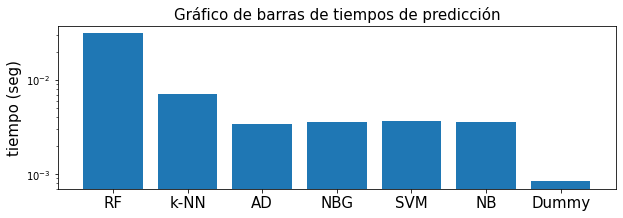
\includegraphics[width=1\textwidth]{grafico_prediccion}
 	\caption{Gráfico de barras con los tiempos medios de predicción de cada modelo.}
 	\label{fig:grafico_prediccion}
\end{figure}
 
 Nuevamente, el clasificador Random Forest lidera la tabla de tiempos, con mucha diferencia del segundo. Esto se debe por la misma razón que en el entrenamiento, es decir, que se trata de un \textit{ensemble}, pues debe realizar varias predicciones con varios árboles de decisión para poder obtener la mejor. Sin embargo, el tiempo medio es muy inferior al anterior, ya que en general, los clasificadores tardan más en construirse que en realizar la predicción. 
 
 Además, vuelve a destacar el clasificador Dummy, con un tiempo medio muy similar al de entrenamiento. El tiempo que tarda en clasificar es prácticamente insignificante, ya que la única tardanza que tiene es la de asignar a cada instancia la clase mayoritaria.
 
 Sin embargo, estos tiempos son prácticamente insignificantes, ya que el clasificador más lento (\textit{i. e.} el Random Forest) tardaría menos de un segundo en entrenar y predecir utilizando este conjunto de ejemplos.
 
 \subsection{Aplicación web}
Uno de los objetivos propuestos en este trabajo es el de realizar una aplicación web para poder predecir si, dado un vídeo de una mano de una persona, esa persona tiene Parkinson o no. Sin embargo, como se ha explicado en puntos anteriores, esta predicción no va a poder ser realizada de la forma ideal, debido a que el conjunto de datos no es demasiado completo como para poder entrenar un clasificador capaz de mostrar una gran diferencia  entre varios niveles de Parkinson. Actualmente, la aplicación predirá entre un 40 y un 50 \% en caso de no tener Parkinson, y entre un 80 y un 90 \% en caso opuesto.

En los resultados de la predicción, se ha destacado el área bajo la curva del clasificador Random Forest, que era superior a la del resto de los clasificadores. Por esta razón, se ha optado por utilizar este clasificador para realizar las predicciones en la aplicación web. No obstante, este modelo puede ser cambiado por el administrador en cualquier momento.

Cualquier vídeo puede ser procesado en la aplicación, siempre y cuando aparezca una mano de forma clara, esta no se salga del vídeo en ningún momento y realice un mínimo de 5 movimientos. Lo ideal para que la aplicación realice la predicción de la forma más rápida y eficaz, sería hacer 10 movimientos, ya que la aplicación escoge los 5 primeros movimientos y los 5 últimos y no tiene en cuenta los movimientos intermedios. Sin embargo, un vídeo con más movimientos podría notar una fatiga en la diferencia entre los 5 primeros movimientos y los 5 últimos, pudiendo afectar en la predicción. Si únicamente se realizan 5 movimientos, la aplicación estaría escogiendo los mismos 5 movimientos ambas veces, y por esta razón, no puede haber menos de 5 movimientos. Además, el número de fotogramas afecta al tiempo de procesado del vídeo, por lo que 5 movimientos realizados de forma lenta tardarán más en procesarse que 5 movimientos realizados de forma más rápida.

Dado que el \textit{software} realizado es una aplicación web, este puede ser utilizado desde dispositivos móviles. Por esta razón, se ha implementado una interfaz diferente para pantallas menores a una anchura, por lo que el menú será más cómodo de utilizar en dispositivos de pantallas pequeñas.
